\documentclass[12pt]{article}  % [12pt] option for the benefit of aging markers
\usepackage{amssymb,amsthm}    % amssymb package contains more mathematical symbols
\usepackage{graphicx}          % graphicx package enables you to paste in graphics
\usepackage[document]{ragged2e} 
\usepackage{float}
\usepackage{tabularx}

%%%%%%%%%%%%%%%%%%%%%%%%%%%%%%%%%
%
%    Page size commands.  Don't worry about these
%
\setlength{\textheight}{220mm}
\setlength{\topmargin}{-10mm}
\setlength{\textwidth}{150mm}
\setlength{\oddsidemargin}{0mm}

%%%%%%%%%%%%%%%%%%%%%%%%%%%%%%%%%%%%%%%%%%%%%%%%%%%%%%%%%%%%%%%
%
%    Definitions of environments for theorems etc.
%
\newtheorem{theorem}{Theorem}[section]          % Theorems numbered within sections - eg Theorem 2.1 in Section 2.
\newtheorem{corollary}[theorem]{Corollary}      % Corollaries etc. will be counted as Theorems for numbering
\newtheorem{lemma}[theorem]{Lemma}              % eg Lemma 3.1, ... Theorem 3.2, ... Corollary 3.3.
\newtheorem{proposition}[theorem]{Proposition}
\newtheorem{conjecture}[theorem]{Conjecture}

\theoremstyle{definition}
\newtheorem{definition}[theorem]{Definition}

\theoremstyle{remark}
\newtheorem{remark}[theorem]{Remark}
\newtheorem{example}[theorem]{Example} 
\graphicspath{ {./Images/} }

%%%%%%%%%%%%%%%%%%%%%%%%%%%%%%%%%%%%%%%%%%%%%%%
%
%        Preamble material specific to your essay
%
\title{Logic-Based Solutions to Puzzles and Riddles\\
Deliverable 1: Research Report}
\author{Kyle Dick\\
F20PA Project\\
supervised by
Kathrin Stark}

\begin{document}
\maketitle

\newpage                     % optional page break
\begin{abstract}
Describe the problem that is to be approached.


\end{abstract}

\newpage                     % optional page break
\tableofcontents

\newpage                     % optional page break
\section{Introduction}\label{s:intro}
%
%In recent times a global interest has developed around the linguistic game Wordle. The concept of this puzzle is simple, the user is to guess a five letter word in as few guesses as possible within six attempts. After each guess the computer will inform the user if a letter was in the correct position, denoted as a green highlight, or is contained within the word but not in the correct %position, denoted with a yellow highlight.
The main focus of this project is to investigate solutions to the puzzle game known as Mastermind. The approach will be to develop an initial base solution in a functional programming language which can be iteratively improved with the goal of creating a solution which is logically sound and efficient.
Mastermind is a simple code-breaking game in which one player will create a secret code which conists of four coloured pegs from a choice of six. This is the standard version of the game however there are multiple variations of the game, some of which will be discussed and examined within the scope of this project.

\subsection {Aims and Objectives}
The aims and objectives of this project can be surmised in two specific goals. The first goal is to derive a solution to the logical puzzle Mastermind. The second goal is to evaluate solutions implemented during this project with the aim to find methods to improve later iterations. An in depth explanation of the chosen aims and objectives are as such:
\begin {itemize}
\item{Aim 1: To derive a solution to the puzzle Mastermind. The goal to find a solution to the problem which minimizes the number of guesses required to discover the correct combination of pegs which comprise the code. Intially the goal will be to derive a base solution to the Mastermind puzzle. The base solution being the most intuitive solution to the problem which does not aim to be the most efficient but to provide a foundation on which improvements can be made.}
	\begin {itemize}
	\item{Objective 1.A: The Mastermind puzzle has previously been the subject of similar research regarding the ability to efficiently find the correct code combination. This stage of the project will concern itself with investigating these previous implementations to guide the project. Through exploring the methods utilised in other investigations into this problem the areas in which these solutions are lacking or could be improved can be found.}
	\item{Objective 1.B:  The ideal base solution should acheive the basic goal of arriving at the correct code combination but should not be the most elegant solution at this point. Instead the base solution should be the foundation for which improvements are made in later iterations. The base solution will be guided through the research conducted through objective 1.A.}
	\item{Objective 1.C: This objective is a continous process which will be referred to throughout the life cycle of the project. Each iteration of the solution, starting with the base solution, should be evaluation against a set of criteria defined later in the document. After this review possible improvements can be documented and worked towards for the next iteration.}
	\end {itemize}
\item{Aim 2: The goal of this project is to arrive at a solution which can be evaluated in terms of its soundness and efficiency. This means that the solution should be one that is easily understood with the appropriate explanation. The steps in which the solution is arrived at should follow a logical progression that is reflected in its documentation. The efficiency should be measured through how quickly the correct code combination can be found by the solution.}
	\begin {itemize}
	\item{Objective 2.A: Designing an evaluation process for this project should be foremost conernced with how well the solution is able to solve the problem. The Mastermind puzzle is most commonly restricted by the amount of guesses allowed to the player. From this the metric in which a solution should be measured against is how quickly the correct code combination can be found and its minimum amount of guesses to do so. A solution which does not reach the correct code combination within a set amount of allowed guesses will be considered a failed solution.}
	\item{Objective 2.B: Analyse an iteration using the chosen strategy.}
	\item{Objective 2.C: Report the results of the evaluation strategy and iterate if improvements are identified.}
	\item{Objective 2.D: Document results taken to arrive at a desired solution.}   
	\end {itemize}
\end {itemize}


%
% The \label command is optional, but useful.  To cross-refer to a section/theorem/equation etc.
% labelled by \label{key}, use \ref{key}.  For example: Equation (\ref{eq:key}) follows from Theorem \ref{th:key}.

\newpage                     % optional page break
\section{Background}\label{ss:back}

This section will provide background material which aims to give context to the aims and objectives of this project. The project was inspired by a paper exploring sudoku solutions from a series of problems known as functional pearls, the processes used to derive those solutions will be used to guide this project in this current stage. Following this brief introduction is an explanation of the game Mastermind which the solution will be derived from along with references to previous work by others. The previous work will relate to the field of functional programming and the specific area of logic and equational reasoning. At the conclusion of this section the goal is that the reader has an understanding of the important concepts relating to this project such that the aims and objectives are clear in their feasability and relevancy.

\subsection {Functional Pearls}
The inspiration for this project was a paper by Richard Bird which implemented a solution to the puzzle game Sudoku as an example of a series of problems known as functional pearls. This sections will explore the topic of functional pearls and their relevance to the current project. Functional Pearls begin as small problems which programmers wish to explore, focusing on brief but engaging examples that showcase either a guided explanation to a proof or presenation of unique data structures. The goal of a functional pearl is to teach important programming techniques and fundamental design principles \cite{Pearls}.  Richard Bird described functional pearls in a speech as 'elegant, instructive exampels of functional programming' while showcasing his implementation of a sudoku solution\cite {R. Bird Speech}.

The solution which this project aims to explore would enter the scope of a functional pearl due to its aim to document an example of functional programming. The project would however deviate from a traditional functional pearl as the scope would be expanded to consider similar solutions in the problem space to evaluate the different methods of solving Mastermind.

The functional pearl which inspired the project is Richard Birds paper 'Functional Pearl: A Program to Solve Sudoku' \cite{Sudoku}. The aim of the solution was to define the function:

\[ Sudoku :: Board \rightarrow [Board]\]

This function would take an input in the form of a Sudoku board, represented by a matrix of characters, and output a list of possible completed boards. Following this declaration the paper would proceed to use logic and equational reasoning to define the function using the functional language haskell to achieve the solution. Finally Richard Bird was able to arrive at the following definition for his solution:

\[ Sudoku :: Board \rightarrow [Board]\]
\[ Sudoku = map (map head) \bullet search \bullet prune \bullet choices\]

where search, prune and choices representing functions declared earlier in the implementation. This sudoku solutions provide an example of how the mastermind solution this project aimst to implement may be approached. Aiming for a solution that resembles this process of declaring an initial function or set of functions then deriving a defintion for them that can be evaluated through comparison with similar solutions. The next section will examine the problem that this project will aim to solve and the work that has been explored in the area previously.


\subsection {Mastermind}

% A brief history and explanation of the game
The aim of this project is to deliver a solution to the code-breaking board game Mastermind designed by Mordecai Meirowitz and originally manufactured by Invicta Toys and Games \cite{Invicta}. 
The original board game consisted of two players with different roles. Player A would be designated the code-breaker while Player B would attempt to solve the code.

The game was designed around player A selecting a code unknown to player B and player B attempting to break the code.
Player A would first construct the code from a set of six coloured pegs with the code being exactly four pegs in length. There are variants where the size of the set of choices and code length are variable however this describes the standard variant.

A variant of the original mastermind puzzle was explored 

\begin{figure}[H]
\centering
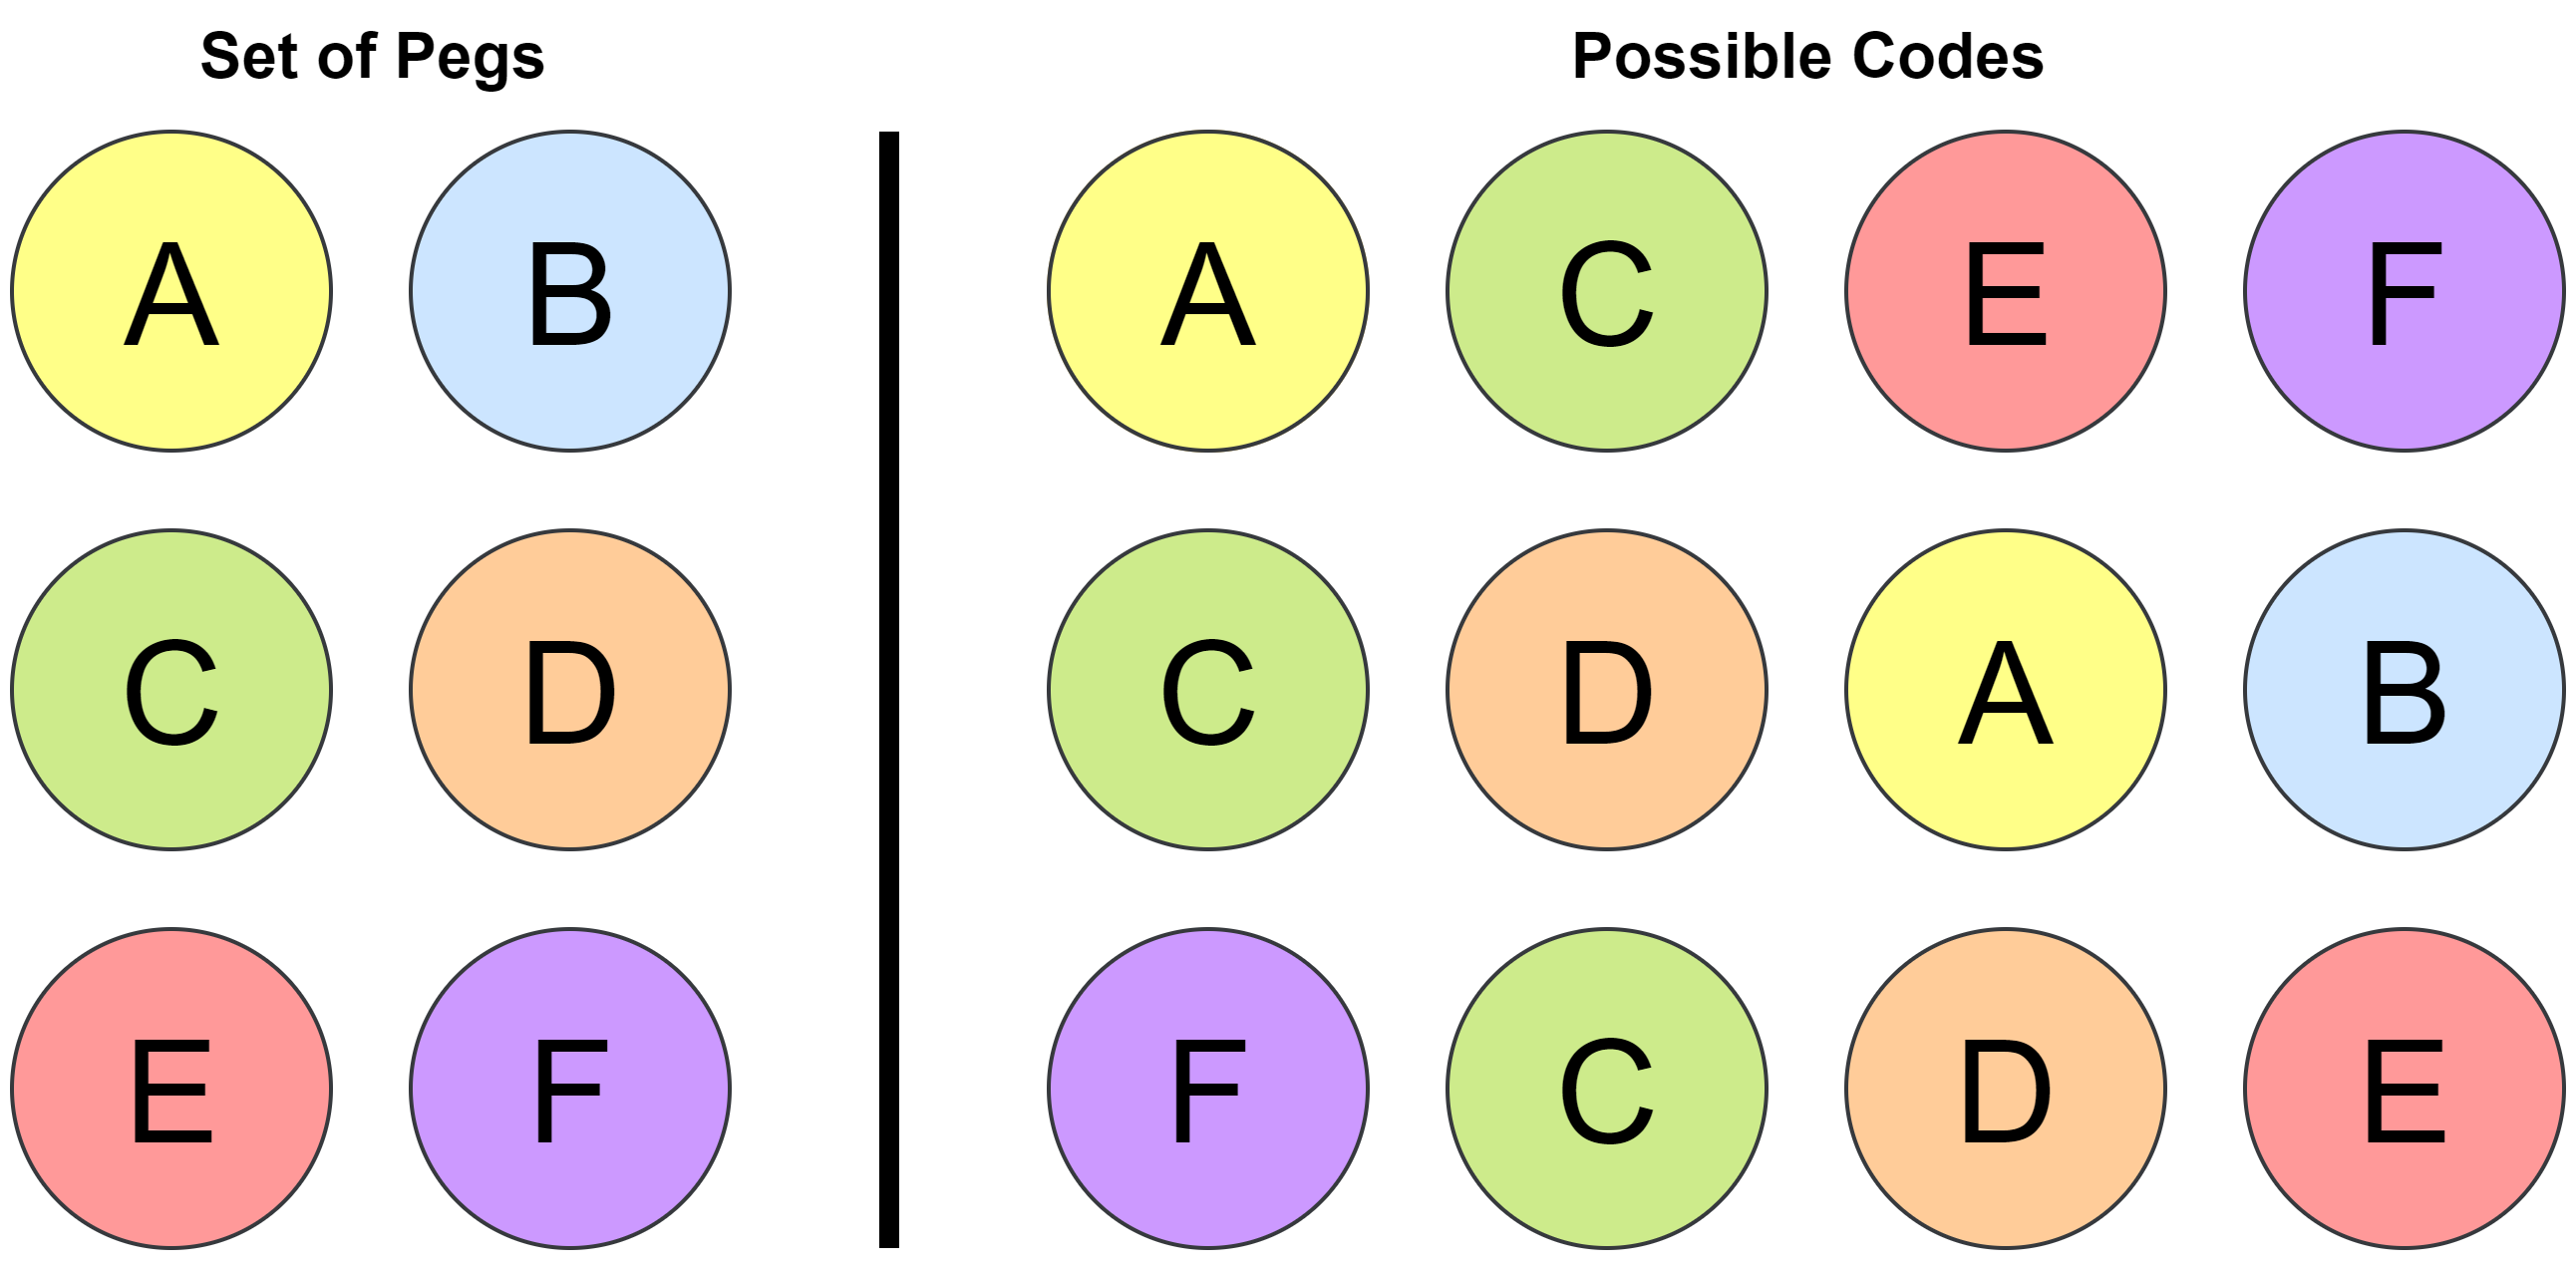
\includegraphics[scale=0.75]{pegs}
\caption{ Example of code enumerations Player A could construct}
\end{figure}

The challenge for Player B is to correctly guess the code created by considering feedback given from Player A relating to how correct each guess was.
A guess is evaluated with Player B given a number of pegs with two possible colours, one which represents a correct position and another which represents a correct colour.

\begin{figure}[H]
\centering
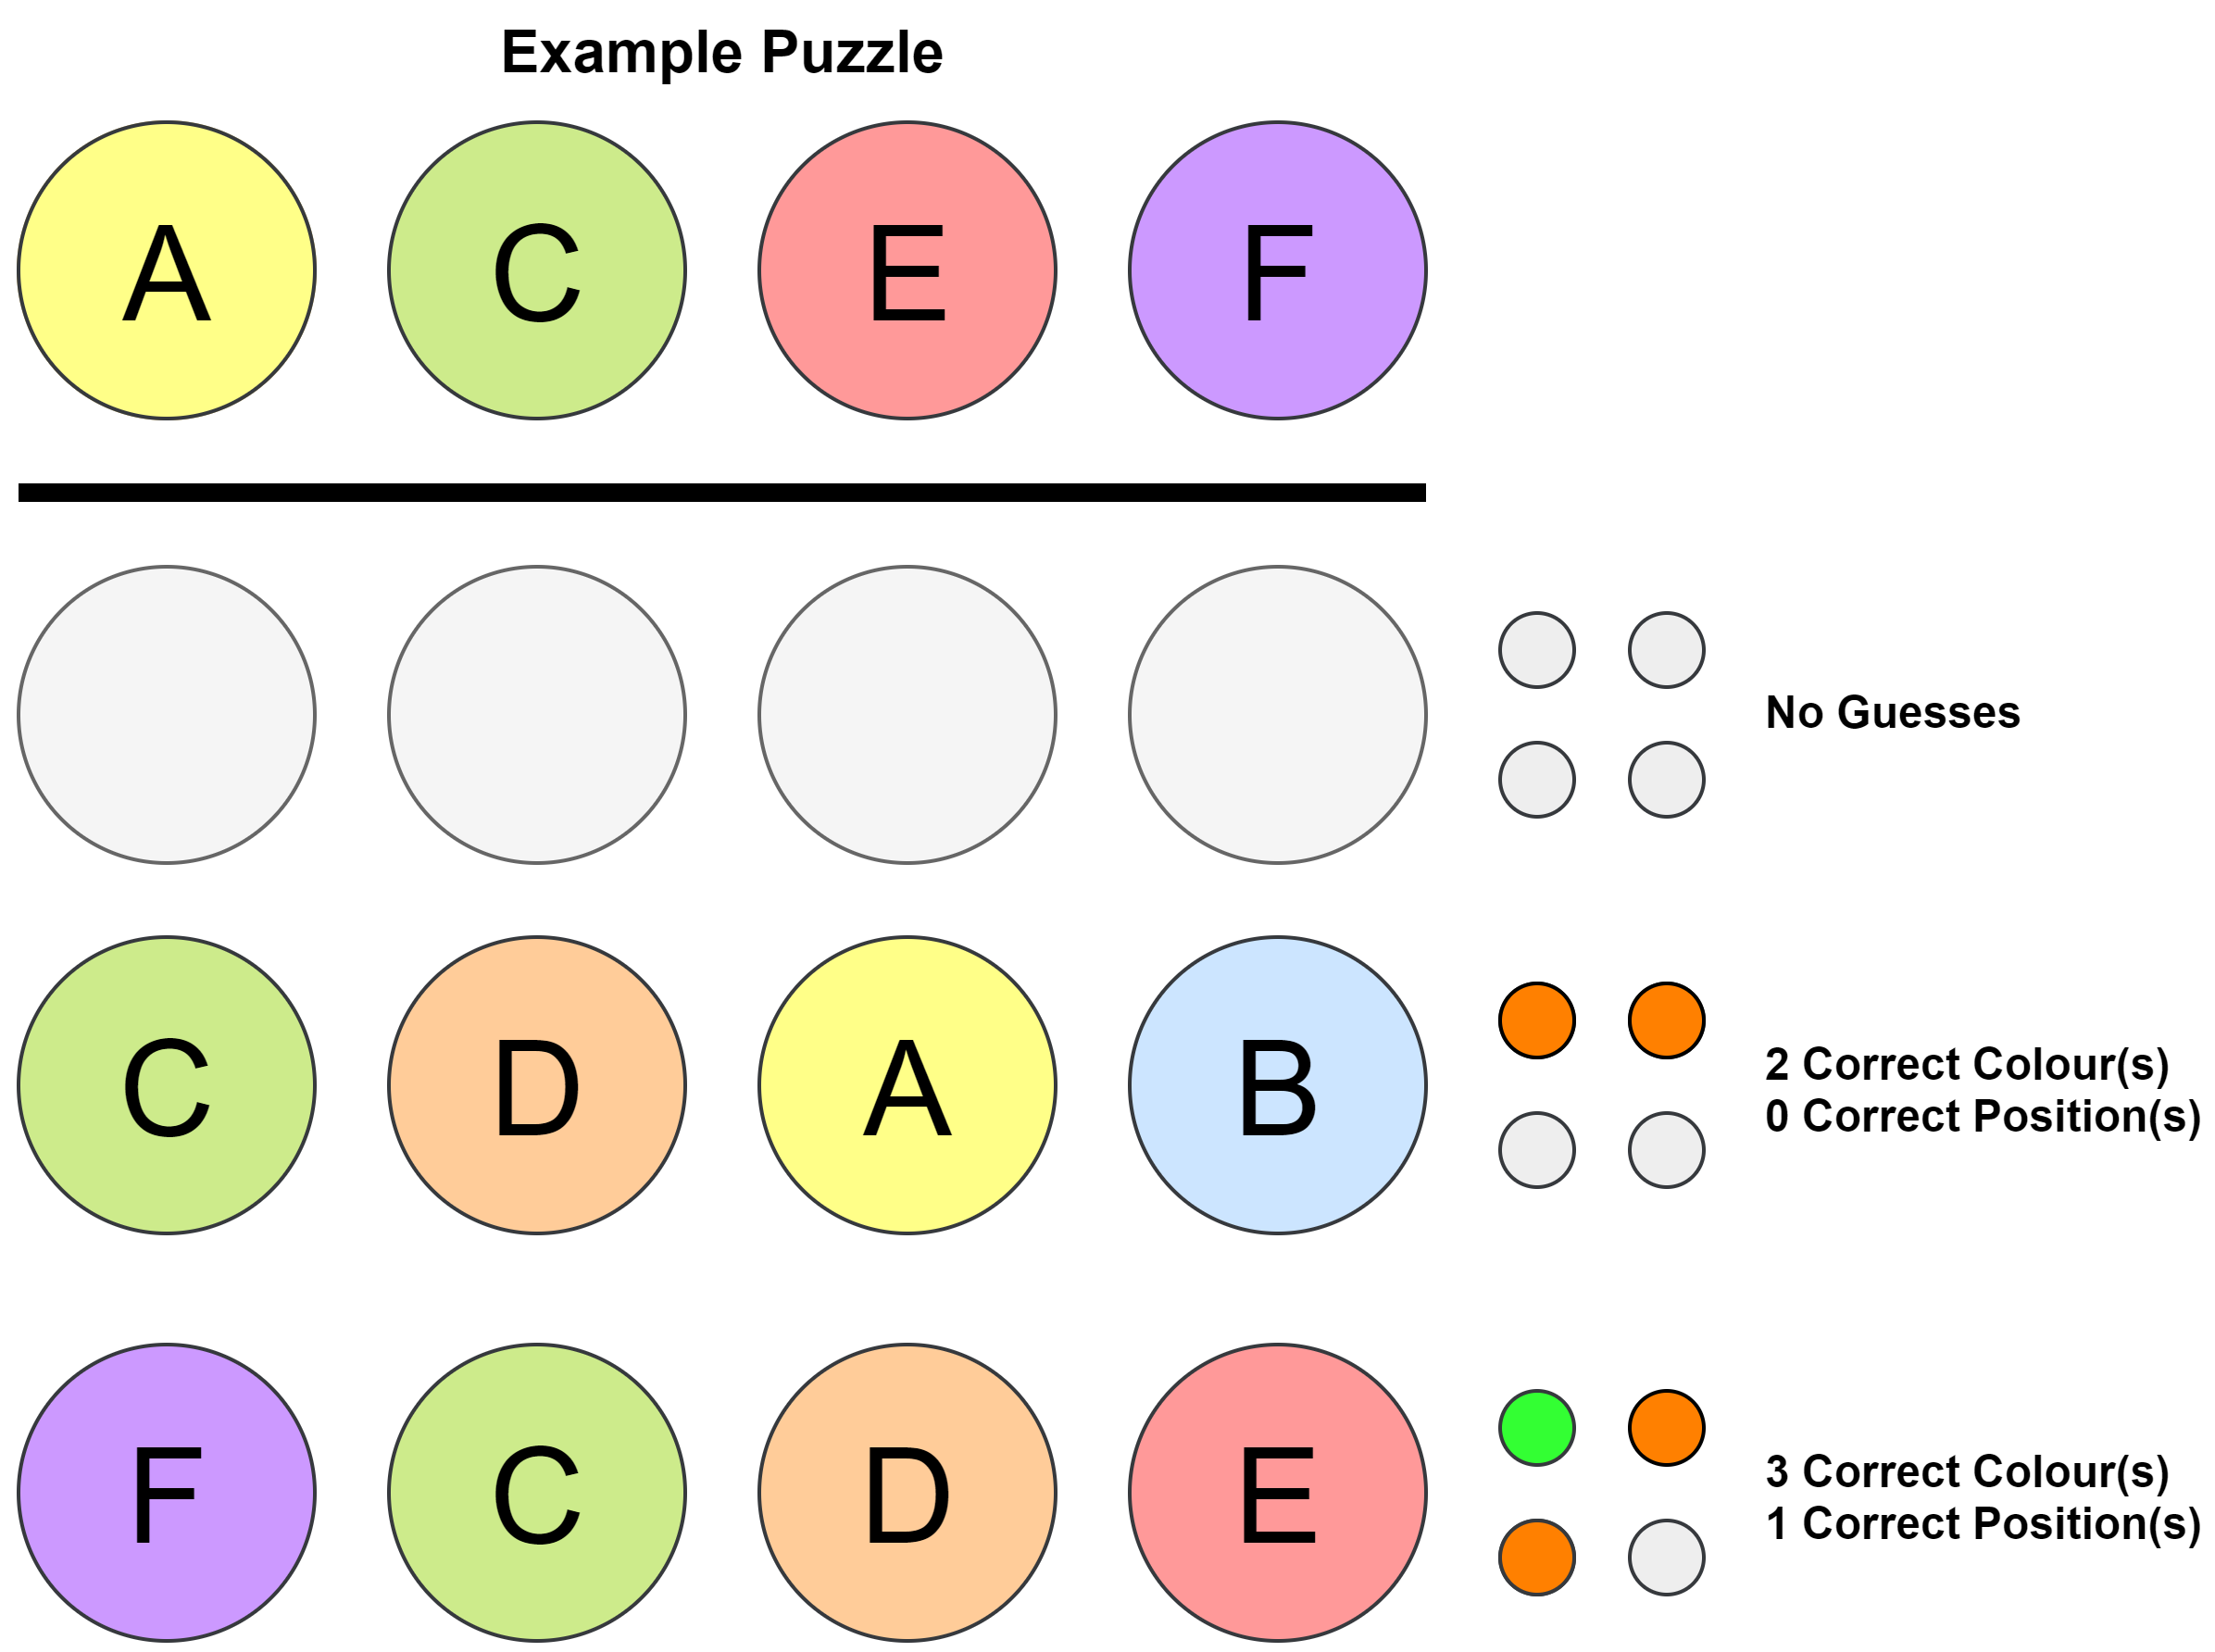
\includegraphics[scale=0.75]{guesses}
\caption{ Simplified example of Player B guesses}
\end{figure}

% A reiteration of the goals with this context
\par The solution that this project aims to implement would assume the role of Player B attempting to correctly identify the generated code in the minimum number of guesses.
To provide a solution which is not bound by the number of elements within the set of possible choices or the length of the code, the code will follow the following rules.

\[ code = [c_i, ... ,c_n]\]
\[pegs = \{c_i, ... , c_m\}\]
\[ n,m = \mathbb{N} > 1\]

% Possible small note about variations and how these could change the goals
A solution which is agnostic of the code length and number of possible elements would support basic variants of Mastermind where the only difference are these restrictions. The base solution will solely focus on solving for a code of length four with six possible elements.

\subsection {Donald Knuth's Solution}

The computer scientist Donald E. Knuth proposed a solution to Master Mind in 1996 which focused on the strategy of minimzing the amount of possible enumerations for the code after each guess. While discussing this he used integers one through six to represent the six possible symbols for the code created by the "codemaker" noting that the total possible number of enumerations being equal to $6^2 = 1296$. 

The first stage of Knuth's investigation was to define the rules of the game in a way that a computer would be able to understand. First defining the two important variables being the code $x_1 x_2 x_3 x_4$ and the test pattern, or guess, $y_1 y_2 y_3 y_4$ The initial rules that were derives were as follows:
\begin {itemize}
	\item {The number of "black hits", i.e., the number of positions j such that $x_j = y_i$}
	\item {The number of "white hits", i.e, the number of positions j such that $x_j =! y_j but x_j = y_k$ for some k and $y_k$ which has not at this point been a hit.} \cite {Knuth}
\end {itemize}

The next step involved defining variables $n_i$ as the number of times symbol i occurs within the codeword and $n'_i$ as the number of times it occurs within the guess for $1 \le i \le 6$. With these variables Knuth was able to define two rules which the computer could understand:

\[1:	 min(n_1, n'_1) + min(n_2, n'_2) + ... + min(n_6, n'_6) \]

for the total number of correct his, both white and black. From this it can be followed that the number of misses is

\[2:	 min(n_1- n'_1, 0) + min(n_2- n'_2, 0) + ... + min(n_6- n'_6, 0) \]

The algorithm that Knuth used would track the remaining possible codes after each test pattern was checked. This would allow Knuth to use the general rule of restricting the number of possible to arrive at the correct code while minimizing the amount of guesses required. Through this method Knuth asserted that it should be possible to achieve a correct guess within five test patterns. The starting pattern discovered by Knuth to give proof to this claim was found to be 1122. A possible progression of stages from this initial test pattern would be:

\[ test \ pattern \ \ \ \  hits \ \ \ \  possbile \ combinations \]
\[ 1122 \ \ \ \ WWW \ \ \ \  16 \]
\[ 1213 \ \ \ \ BWW \ \ \ \  4 \]

This idealistic situation would result in the next test pattern being able to distuingish from the final four possible combinations using the test pattern 1415.
Another example is as follows:

\[ test \ pattern \ \ \ \  hits \ \ \ \  possbile \ combinations \]
\[ 1122 \ \ \ \ B \ \ \ \  256 \]
\[ 1344 \ \ \ \ W \ \ \ \  44 \]
\[ 3526 \ \ \ \ BWW \ \ \ \  7 \]

This situation would also allow for the next test pattern to distuingish the final possible combinations using the test pattern 1462. The algorithm used to decide the progression from one test pattern to next decides based on the test pattern which is able to minimize the number of possible combinations. The algorithm selects the first test pattern such that there is no situation where the fourth test pattern is unable to distuingish the final remaining code combinations giving credit to Knuth's claim that the correct code can be ascertained within five guesses.

This method of solving the problem however is admitted within the paper to not be the most optimal solution. This can be shown by the way that the algorithm processes the following situation:

\[ test \ pattern \ \ \ \  hits\]
\[ 1122 \ \ \ \ BWW\]
\[ 1213 \ \ \ \ BB\]

which results in a possible four remaining code words (2212, 4212, 5212, 6212). The algorithm would select the test pattern 1145 as the next guess however when compared to the test pattern 4222 it can be shown that it in actuality results in less distinguishing results:

\[ 4222: \ \ BBW = 2212 \ \ BBB = 4212 \ \ BB = 5212 \ \ BB = 6212 \]
\[ 1145: \ \ W = 2212 \ \ WW = 4212 \ \ WW = 5212 \ \ W = 6212 \]

It is clear that should 4222 be used at the test pattern there are two possibilities in 2212 and 4212 where the code can be known by the third guess. This is a better result compared to the test pattern 1145 where two possibilities will always be the result.


\subsection {Logic and Equational Reasoning}
% Discussion of what a logical approach to programming would be
The goal with the solution this project aims for is to implement a solution which is logically sound. This means for the project to succeed

% Equational Reasoning vs Maths

\newpage                     % optional page break
\section{Research Methodology}\label{ss:back}

\newpage                     % optional page break
\section{Evaluation Strategy}\label{ss:back}

The evaluation strategy will be concerned mostly with trying to get the minimum amount of guesses within the allowed span of guesses.
In here there will be further discussion of the attempts made in previous studies and their results.

\newpage
\section {Preliminary Work}

In here talk about the work done with the current base solution. It will be originally done based on the donald knuth implementation.


\newpage                     % optional page break
\section{Project Management}\label{ss:back}

\subsection {File and Resource Management}

\subsection {Timeline and Deadlines}

\subsection {Risk Analysis and Mitigations}

To manage the progress of this project efficiently it was important to identify possible risks that could prevent the realisation of the goals laid out earlier in this document. To aid in the identification of the risks the following key was used to classify the associated risks:
\begin{itemize}
\item{People (P) - Risks which are the result of issues related to those individuals involved in the project. This relates to the wellbeing, scheduling and personal issues that can be encountered.}
\item{Technological (T) - Risks which can result from the technology being used to engineer the solutions. This relates to the technologial constraints that could be encountered or the hardware required.}
\item{Requirement (R)  - Risks which can result from changes to the requirements of the project. This relates to problems encountered with the work being implemented for the project. Logical problems and issues with the material involved would be included in these risks.}
\end{itemize}

\begin{tabularx}{1.1\textwidth} {
	|  >{\center\arraybackslash}X
	| >{\center\arraybackslash}X
	| >{\center\arraybackslash}X
	| >{\center\arraybackslash} X | }
	\hline
	ID & Risk & Description \\
	\hline
	P/T/R1 & Textual Title of Risk & Textual Description of the Risk \\
	\hline
\end{tabularx}

\begin{tabularx}{1.1\textwidth} {
	|  >{\center\arraybackslash}X
	| >{\center\arraybackslash}X
	| >{\center\arraybackslash}X
	| >{\center\arraybackslash} X | }
	\hline
	ID & Risk & Description \\
	\hline
	P.1 & Illness and Health Complications & The situation in which an individual involved in the project is unable to contribute due to illness or health complications. This risk is slightly heightened as the world recovers from the effects of the Covid-19 pandemic however it also considers other conditions which would require time away from the project. \\
	\hline
	T.1 & File Loss & This is the situation in which files or documents relating to the project is lost. This is a low priority issue as precautions have been taken to mitigate this such as using version control through Github. \\
	\hline
	R.1 & Insufficient Base Solution & The success of this project is dependant on having a solid base solution. The success of the base solution is assessed by a set of conditions which deems it suitable for solving the problem. The base solution being unable to meet this conditions is a serious situation and as such should be of a high priority. \\
	\hline
\end{tabularx}



%%%%%%%%%%%%%%%%%%%%%%%%%%%%%%%%%%%%%%%%%
%
%     Bibliography
%
%     Use an easy-to-remember tag for each entry - eg \bibitem{How97} for an article/book by Howie in 1997
%     To cite this publication in your text, write \cite{How97}.  To include more details such as
%     page, Chapter, Theorem numbers, use the form \cite[Theorem 6.3, page 42]{How97}.
%
\begin{thebibliography}{99}

% 
% The usual convention for mathematical bibliographies is to list alphabetically
% by first-named author (then second, third  etc. author then date)
% websites with no author names should go by the site name
%

% Typical layout for reference to a journal article
%\bibitem{Bovey}
%J. D. Bovey, M. M. Dodson,                         % author(s)
%The Hausdorff dimension of systems of linear forms % article name
%{\em Acta Arithmetica}                             % journal name - italics
%{\bf 45}                                           % volume number - bold
%(1986), 337--358.                                   % (year), page range


% Typical layout for reference to a book
%
%\bibitem{Cassels}
%J. W. S. Cassels,                                  % author(s)
%{\em An Introduction to Diophantine Approximation},% title - italics
%Cambridge University Press, Cambridge, 1965.       % Publisher, place, date.

% Typical layout for reference to a website
%
%\bibitem{GAP}
%The GAP Group, GAP -- Groups, Algorithms, and Programming,  % Site name
%Version 4.5.6; 2012. % other information
%(http://www.gap-system.org)  % URL


% Typical layout for reference to an online article

%\bibitem{Howie}
%J. Howie,                                            % author(s)
%{\em Generalised triangle groups of type $(3,5,2)$}, % article name - italics
%http://arxiv.org/abs/1102.2073                       % URL
%(2011).                                              % (year)

\bibitem {Pearls}
Richard Bird,
{\em How to Write a Functional Pearl}
International Conference on Functional Programming, Portland
(2006)

\bibitem {R. Bird Speech}
Jeremy Gibbons,
{\em University of Oxford, Functional Pearls}
http://www.cs.ox.ac.uk/people/jeremy.gibbons/pearls/
(2009)

\bibitem {Sudoku}
Richard Bird
{\em Functional Pearl, A Program to Solve Sudoku}
Cambridge University Press, Cambridge, 2006

\bibitem {Invicta}
Invicta Toys and Games ltd,
{\em History of Mastermind}
https://web.archive.org/web/20070812104420/http://dspace.dial.pipex.com/town/road/gbd76/toys.htm
(Archived 2007)

\bibitem {Knuth}
Donald E. Knuth,
The Computer as Master Mind
{\em Recreational Mathematics}
{\bf 9(1)}
(1976)

\end{thebibliography}
\end{document}
